%%%%%%%%%%%%%%%%%%%%%%%%%%%%%%%%%%%%%%%%%
% Short Sectioned Assignment LaTeX Template Version 1.0 (5/5/12)
% This template has been downloaded from: http://www.LaTeXTemplates.com
% Original author:  Frits Wenneker (http://www.howtotex.com)
% License: CC BY-NC-SA 3.0 (http://creativecommons.org/licenses/by-nc-sa/3.0/)
%%%%%%%%%%%%%%%%%%%%%%%%%%%%%%%%%%%%%%%%%

%----------------------------------------------------------------------------------------
%	PACKAGES AND OTHER DOCUMENT CONFIGURATIONS
%----------------------------------------------------------------------------------------

\documentclass[paper=a4, fontsize=11pt]{scrartcl} % A4 paper and 11pt font size

% ---- Entrada y salida de texto -----

\usepackage[T1]{fontenc} % Use 8-bit encoding that has 256 glyphs
\usepackage[utf8]{inputenc}
%\usepackage{fourier} % Use the Adobe Utopia font for the document - comment this line to return to the LaTeX default

% ---- Idioma --------

\usepackage[spanish, es-tabla]{babel} % Selecciona el español para palabras introducidas automáticamente, p.ej. "septiembre" en la fecha y especifica que se use la palabra Tabla en vez de Cuadro

% NOTA: en caso de problema al compilar, compruebe que tiene el paquete: texlive-babel-spanish.noarch

% ---- Otros paquetes ----

\usepackage{amsmath,amsfonts,amsthm} % Math packages
\usepackage{graphics,graphicx,floatrow} %para incluir imágenes y notas en las imágenes
\usepackage{listings}

\usepackage{url}

%% Define a new 'leo' style for the package that will use a smaller font.
\makeatletter
\def\url@leostyle{%
	\@ifundefined{selectfont}{\def\UrlFont{\sf}}{\def\UrlFont{\small\ttfamily}}}
\makeatother
%% Now actually use the newly defined style.
\urlstyle{leo}
\setlength{\parindent}{12pt}

% Para hacer tablas comlejas
\usepackage{multirow}
\usepackage{threeparttable}

%\usepackage{sectsty} % Allows customizing section commands
%\allsectionsfont{\centering \normalfont\scshape} % Make all sections centered, the default font and small caps

\usepackage{fancyhdr} % Custom headers and footers
\pagestyle{fancyplain} % Makes all pages in the document conform to the custom headers and footers
\fancyhead{} % No page header - if you want one, create it in the same way as the footers below
\fancyfoot[L]{} % Empty left footer
\fancyfoot[C]{} % Empty center footer
\fancyfoot[R]{\thepage} % Page numbering for right footer
\renewcommand{\headrulewidth}{0pt} % Remove header underlines
\renewcommand{\footrulewidth}{0pt} % Remove footer underlines
\setlength{\headheight}{13.6pt} % Customize the height of the header

\numberwithin{equation}{section} % Number equations within sections (i.e. 1.1, 1.2, 2.1, 2.2 instead of 1, 2, 3, 4)
\numberwithin{figure}{section} % Number figures within sections (i.e. 1.1, 1.2, 2.1, 2.2 instead of 1, 2, 3, 4)
\numberwithin{table}{section} % Number tables within sections (i.e. 1.1, 1.2, 2.1, 2.2 instead of 1, 2, 3, 4)

\setlength\parindent{0pt} % Removes all indentation from paragraphs - comment this line for an assignment with lots of text

\newcommand{\horrule}[1]{\rule{\linewidth}{#1}} % Create horizontal rule command with 1 argument of height



\usepackage[utf8]{inputenc}
\usepackage[T1]{fontenc}
\usepackage[spanish]{babel}
\usepackage{times}

\usepackage{color}
\definecolor{gray97}{gray}{.97}
\definecolor{gray75}{gray}{.75}
\definecolor{gray45}{gray}{.45}

\usepackage{listings}
\lstset{ frame=Ltb,
	framerule=0pt,
	aboveskip=0.5cm,
	framextopmargin=3pt,
	framexbottommargin=3pt,
	framexleftmargin=0.4cm,
	framesep=0pt,
	rulesep=.4pt,
	backgroundcolor=\color{gray97},
	rulesepcolor=\color{black},
	%
	stringstyle=\ttfamily,
	showstringspaces = false,
	basicstyle=\small\ttfamily,
	commentstyle=\color{gray45},
	keywordstyle=\bfseries,
	%
	numbers=left,
	numbersep=15pt,
	numberstyle=\tiny,
	numberfirstline = false,
	breaklines=true,
}

% minimizar fragmentado de listados
\lstnewenvironment{listing}[1][]
{\lstset{#1}\pagebreak[0]}{\pagebreak[0]}

\lstdefinestyle{consola}
{basicstyle=\scriptsize\bf\ttfamily,
	backgroundcolor=\color{gray75},
}

\lstdefinestyle{C}
{language=C,
}


\usepackage[pdftex,colorlinks=true,linkcolor=negro,urlcolor=blue]{hyperref,xcolor}
\definecolor{negro}{rgb}{0,0,0}

\graphicspath{ {./imagenes/} }
\usepackage{subfig}
\hypersetup{citecolor=blue}

\title{	
\normalfont \normalsize 
\textsc{{\bf Ingeniería de Servidores (2014-2015)} \\ Grado en Ingeniería Informática \\ Universidad de Granada} \\ [25pt]
\horrule{0.5pt} \\[0.4cm] % Thin top horizontal rule
\huge Memoria Prácticas Opcionales \\ % The assignment title
\horrule{2pt} \\[0.5cm] % Thick bottom horizontal rule
}

\author{Jose Antonio Jiménez Montañés}

\date{\normalsize\today}

%----------------------------------------------------------------------------------------
% DOCUMENTO
%----------------------------------------------------------------------------------------
%
%\begin{figure}[H]
%	\centering
%	\includegraphics[width=0.5\textwidth]{gull}
%	\caption{Texto Prueba}
%	\label{fig:ddd}
%\end{figure}


%\cite{p1}


\begin{document}

\maketitle % Muestra el Título

\newpage %inserta un salto de página

\tableofcontents % para generar el índice de contenidos
\clearpage
\listoffigures

%\listoftables 

\newpage

%----------------------------------------------------------------------------------------
% CUESTION OPCIONAL 1
%----------------------------------------------------------------------------------------
\section{Muestre (con capturas de pantalla) como ha comprobado que el RAID1 funciona}

Consultando el archivo /proc/mdstat. Si los 2 discos RAID están funcionando correctamente el sistema raid se marcará con una doble U (‘UU’) si alguno fallase mostraría solo una U con una barra baja en el lugar del disco con fallo (‘\_U’).\\
\begin{figure}[H]
	\centering
	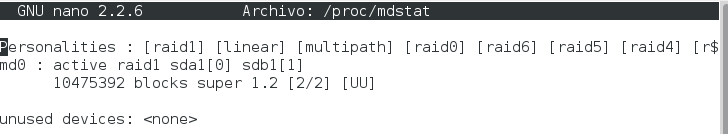
\includegraphics[width=1\textwidth]{1/op1}
	\caption{Comprobación del estado del RAID1}
	\label{fig:f01}
\end{figure}


%------------------------------------------------
% CUESTION OPCIONAL 2
%------------------------------------------------
\section{¿Que relación hay entre los atajos de teclado de emacs y los de la consola bash?.¿y entre los de vi y las paginas del manual?}

Los atajos de emacs son casi idénticos a los de bash ya que es desarrollado por GNU aunque se puede cambiar la configuración al estilo Vi/Vim escribiendo:  ‘set –o vi’.\\

Los atajos de las páginas del manual son idénticos a los del vi aunque internamente parece que no tienen que ver ya que las "man pages" no se basan en vi sino en "boost".


%-------------------------------------------------------------------------------------------
% CUESTION OPCIONAL 3
%--------------------------------------------------------------------------------------------
\section{¿Que gestores utiliza OpenSuse?}

De manera gráfica utiliza YaST, y para el modo consola utiliza Zypper.

\clearpage
%----------------------------------------------------------------------------------------
% CUESTION OPCIONAL 4
%----------------------------------------------------------------------------------------
\section{Instale y pruebe terminator. Con screen, pruebe su funcionamiento dejando sesiones ssh abiertas en el servidor y recuperándolas posteriomente.}

Primero ya que estoy trabajando con Centos he tenido que descargar el rpm con terminator de: http://li.nux.ro/download/nux/dextop/el7/x86\_64/terminator-0.97-6.el7.nux.noarch.rpm \\

Luego he instalado las 3 dependencias que son necesarias para instalar el rpm de terminator que son:\\

\begin{figure}[H]
	\centering
	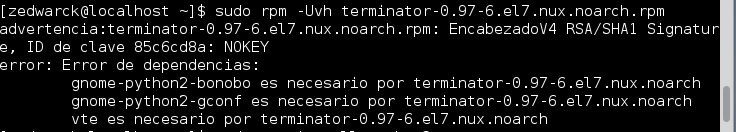
\includegraphics[width=1\textwidth]{2/co02f01}
	\caption{Dependencias faltantes para instalar rpm de terminator}
	\label{fig:f02}
\end{figure}

Finalmente se instala el comando screen con: yum install screen. NOTA: Puede que se necesite tener los repositorios EPEL instalados. \cite{c01} \\

Ya se puede acceder desde la sesión SSH al comando screen para que nos virtualice una sesión de terminal que no se cerrara en caso de desconexión del túnel ssh. \\
Si se desconecta se puede ver las sesiones virtuales abiertas con screen -ls y acceder a una de ellas usando su ID con screen -r <ID> \cite{c02} \\

\begin{figure}[H]
	\centering
	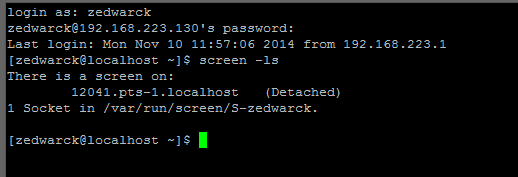
\includegraphics[width=1\textwidth]{2/co02f02}
	\caption{Uso del comando screen}
	\label{fig:f03}
\end{figure}


%----------------------------------------------------------------------------------------
% CUESTION OPCIONAL 5
%----------------------------------------------------------------------------------------
\section{Instale el servicio fail2ban y pruebe su funcionamiento.}

Primero instalamos el paquete con yum install fail2ban \\

\begin{figure}[H]
	\centering
	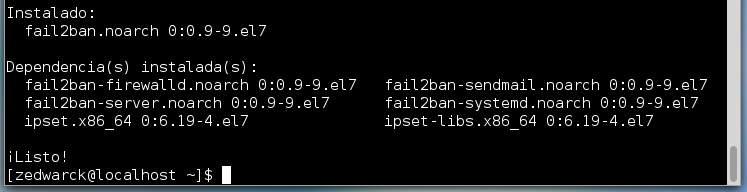
\includegraphics[width=1\textwidth]{2/co03f01}
	\caption{Instalación completada de fail2ban}
	\label{fig:f04}
\end{figure}

Y activamos el servicio y comprobamos que esta ejecutandose: \\

\begin{figure}[H]
	\centering
	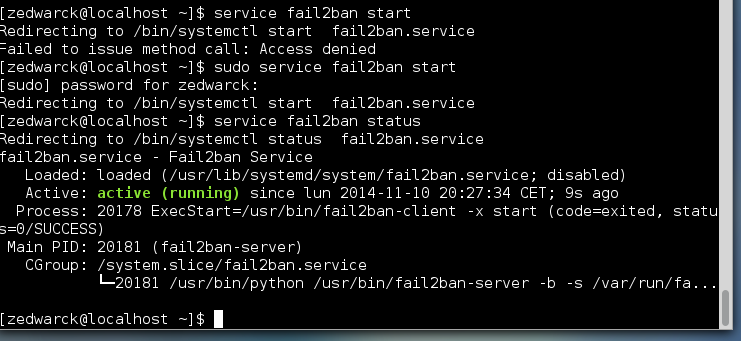
\includegraphics[width=1\textwidth]{2/co03f02}
	\caption{Servicio fail2ban funcionando}
	\label{fig:f05}
\end{figure}


Después solo tendremos que crear el archivo de configuración y configurarlo a nuestro gusto para restringir ciertas IPS, incluso con aviso por email en caso de intento no autorizado. \cite{c03} \\

\clearpage
%----------------------------------------------------------------------------------------
% CUESTION OPCIONAL 6
%----------------------------------------------------------------------------------------
\section{Realice la instalación de uno de estos dos “web containers” y pruebe su ejecución.}

Primero instalamos Java
\begin{figure}[H]
	\centering
	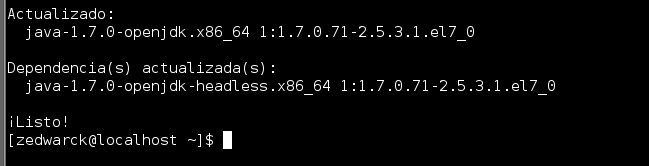
\includegraphics[width=0.8\textwidth]{2/co04f01}
	\caption{Instalación de Java completada}
	\label{fig:f06}
\end{figure}
Luego TomCat 
\begin{figure}[H]
	\centering
	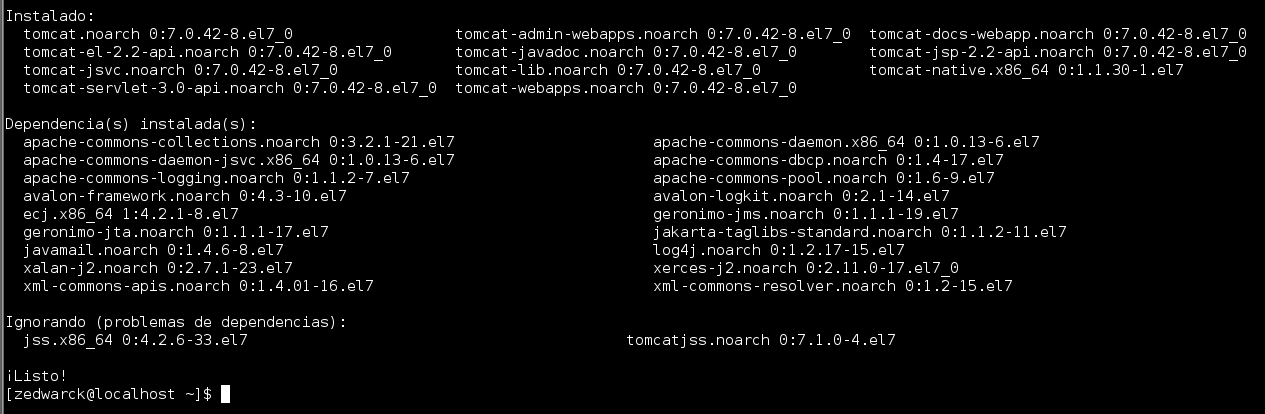
\includegraphics[width=0.8\textwidth]{2/co04f02}
	\caption{Instalación de TomCat completada}
	\label{fig:f07}
\end{figure}

Luego configuramos Tomcat \cite{c04} y probamos poniendo la ip local en el puerto 8080 en el navegador.
\begin{figure}[H]
	\centering
	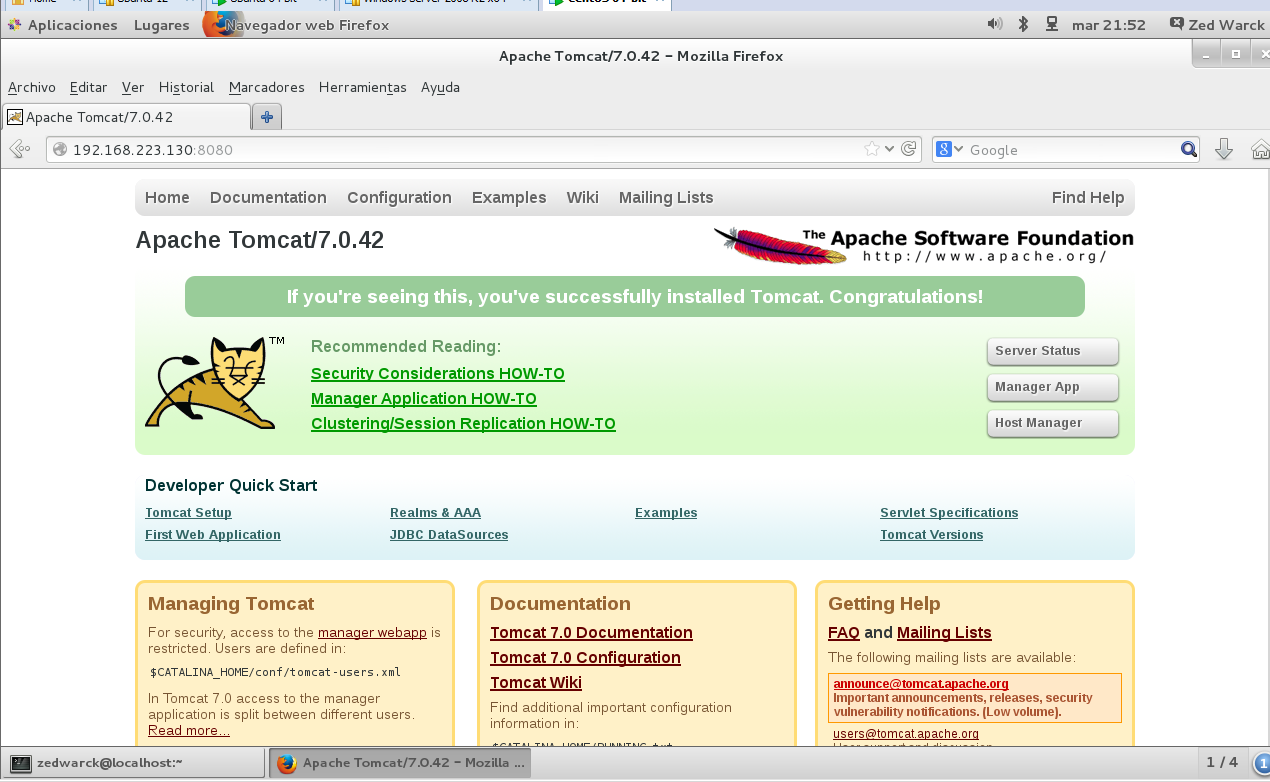
\includegraphics[width=0.6\textwidth]{2/co04f03}
	\caption{Instalación de TomCat probada}
	\label{fig:f08}
\end{figure}


%----------------------------------------------------------------------------------------
% CUESTION OPCIONAL 7
%----------------------------------------------------------------------------------------
\section{Realice la instalación de MongoDB en alguna de sus máquinas virtuales. Cree una colección de documentos y haga una consulta sobre ellos.}

Primero instalamos MongoDB y lo configuramos: \cite{c05} \\
\begin{figure}[H]
	\centering
	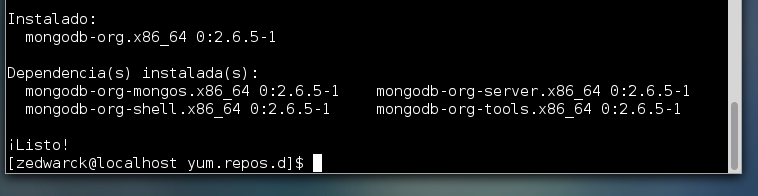
\includegraphics[width=1\textwidth]{2/co05f01}
	\caption{Instalación de MongoDB completada}
	\label{fig:f09}
\end{figure}

Y luego nos conectamos y creamos las colecciones de prueba: \cite{c06} \\
\begin{figure}[H]
	\centering
	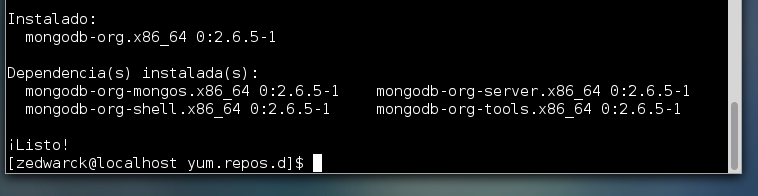
\includegraphics[width=1\textwidth]{2/co05f01}
	\caption{Proceso de creación y consulta de la colección de datos}
	\label{fig:f10}
\end{figure}

\clearpage
%----------------------------------------------------------------------------------------
% CUESTION OPCIONAL 8
%----------------------------------------------------------------------------------------
\section{Indique qué comandos ha utilizado para realizarlo así como capturas de pantalla del proceso de reconstrucción del RAID. \cite{c07}}

Comprobamos primero que funciona el RAID1 y eliminamos el disco2. Comprobamos que detecta que el disco 2 falla: (Lo hemos eliminado)

\begin{figure}[H]
	\centering
	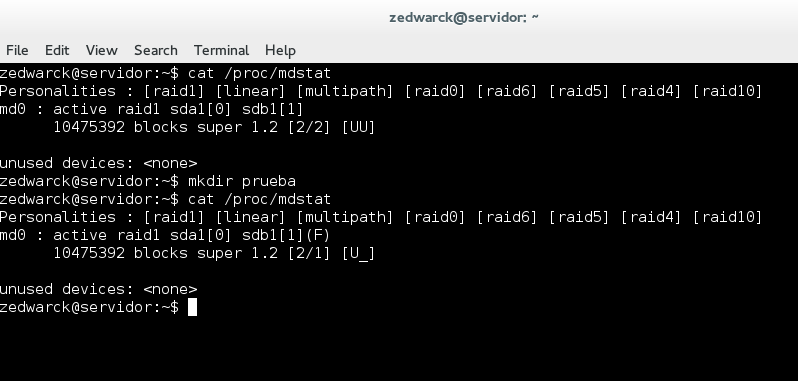
\includegraphics[width=0.8\textwidth]{3/co01f01}
	\caption{Sistema detecta que el RAID falla}
	\label{fig:f11}
\end{figure}


Si el disco diera fallos lógicos debería ser retirado con: "sudo mdadm --remove /dev/md0 /dev/sdb1"\\

De una forma u de otra el siguiente paso sería retirarlo del sistema con: "sudo mdadm --manage /dev/md0 --remove /dev/sdb1"\\

Luego procedemos a instalar el nuevo disco que ya debería estar en el sistema con: "sudo mdadm --add /dev/md0 /dev/sdb1"\\

Comprobamos que ahora esta el disco en el sistema RAID y esta actualizando datos:

\begin{figure}[H]
	\centering
	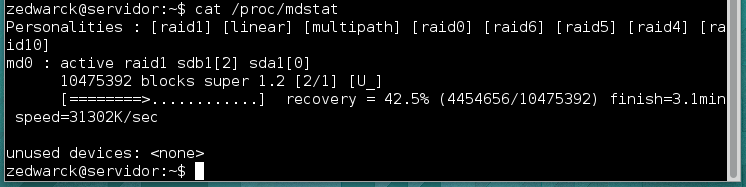
\includegraphics[width=0.8\textwidth]{3/co01f02}
	\caption{Sistema detecta nuevo disco en RAID y lo actualiza}
	\label{fig:f12}
\end{figure}


%----------------------------------------------------------------------------------------
% CUESTION OPCIONAL 9
%----------------------------------------------------------------------------------------
\section{Instale Nagios en su sistema (el que prefiera)	documentando el proceso y muestre el resultado de la monitorización de su sistema comentando qué aparece. \cite{c08}}


Para instalar Nagios en Ubuntu primero preinstalamos algunos requisitos. segun el manual habría que poner:\\

sudo apt-get install wget build-essential apache2 php5-gd libgd2-xpm libgd2-xpm-dev libapache2-modphp5\\

Pero vamos a dejar la linea de la siguiente manera para Ubuntu 14.04:\\

sudo apt-get install wget build-essential apache2 php5-gd libgd2-xpm-dev apache2-utils\\

\begin{figure}[H]
	\centering
	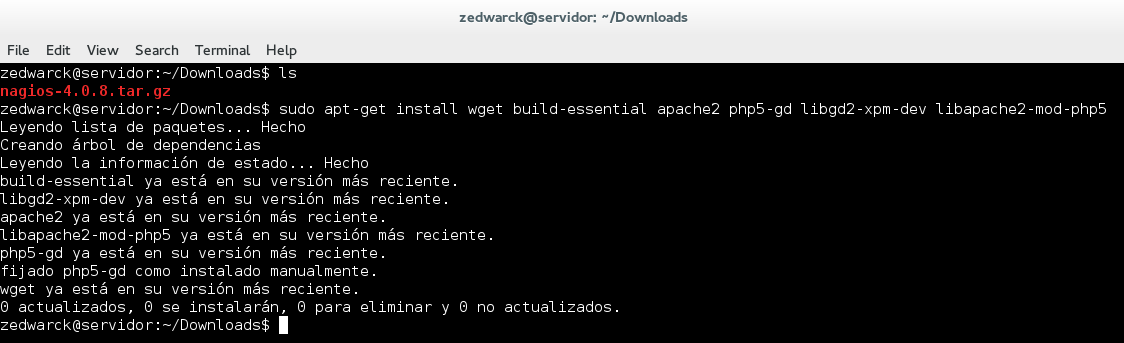
\includegraphics[width=1\textwidth]{3/co02f01}
	\caption{Prerequisitos de nagios con apt-get.}
	\label{fig:f13}
\end{figure}

Luego nos descargamos nagios:\\
cd /tmp\\
wget http://prdownloads.sourceforge.net/sourceforge/nagios/nagios-4.0.4.tar.gz\\
wget http://nagios-plugins.org/download/nagios-plugins-2.0.tar.gz\\

Nos creamos un grupo y un usuario en él que se necesita para su correcto funcionamiento:\\
useradd nagios\\
groupadd nagcmd\\
usermod -a -G nagcmd nagios\\

\begin{figure}[H]
	\centering
	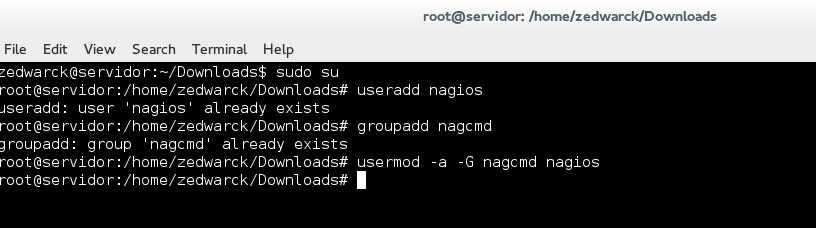
\includegraphics[width=1\textwidth]{3/co02f02}
	\caption{Creacion de usuario y grupo Nagios.}
	\label{fig:f14}
\end{figure}

Descomprimimos:\\
tar zxvf nagios-4.0.4.tar.gz\\
tar zxvf nagios-plugins-2.0.tar.gz\\

\begin{figure}[H]
	\centering
	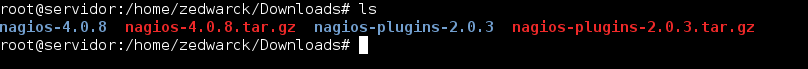
\includegraphics[width=1\textwidth]{3/co02f03}
	\caption{Archivos de instalación de Nagios descomprimidos.}
	\label{fig:f15}
\end{figure}

Accedemos al directorio de instalación y configuramos el instalador:\\

./configure --with-nagios-group=nagios --with-command-group=nagcmd -–with-mail=/usr/bin/sendmail\\

\begin{figure}[H]
	\centering
	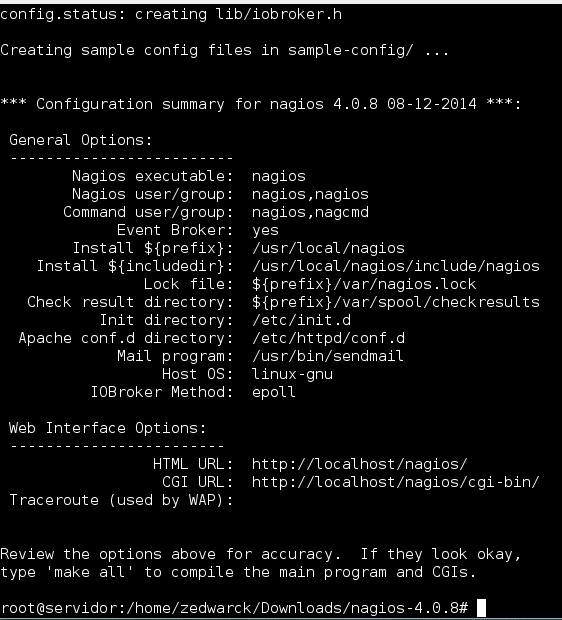
\includegraphics[width=1\textwidth]{3/co02f04}
	\caption{Preconfiguración de Nagios completada.}
	\label{fig:f16}
\end{figure}

Luego hacemos los makes:\\
make all\\
make install\\
make install-init\\
make install-config\\
make install-commandmode\\
make install-webconf\\

\begin{figure}[H]
	\centering
	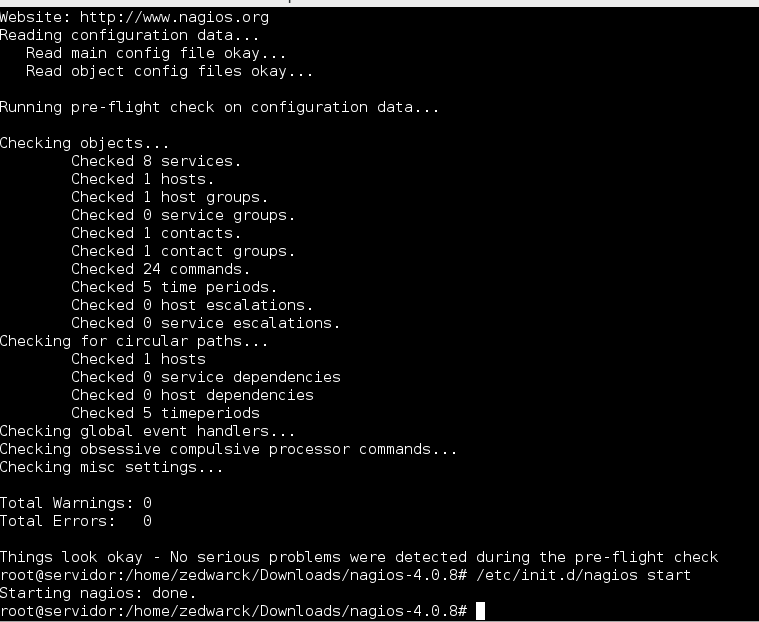
\includegraphics[width=1\textwidth]{3/co02f05}
	\caption{Instalacion de Nagios completada y servicio corriendo.}
	\label{fig:f17}
\end{figure}

El último puede que nos de error, si es así nos creamos el directorio /etc/httpd/conf.d y volvemos a ejecutar el ultimo make. Después de eso nos vamos a ese directorio y copiamos el archivo nagios.conf al directorio de configuraciones de apache: /etc/apache2/conf-enabled/ \\

Finalmente ponemos:\\
cp -R contrib/eventhandlers/ /usr/local/nagios/libexec/ \\
chown -R nagios:nagios /usr/local/nagios/libexec/eventhandlers \\
/usr/local/nagios/bin/nagios -v /usr/local/nagios/etc/nagios.cfg \\

Iniciamos el servicio naglios: service nagios restart \\

Por ultimo reiniciamos apache: service apache2 restart \\


Para poder acceder nos hace falta configurar un usuario:\\

htpasswd –c /usr/local/nagios/etc/htpasswd.users nagiosadmin \\


Y para poder visualizar gráficas nos hace falta el pluging:\\

cd /tmp/nagios-plugins-2.0 \\
./configure --with-nagios-user=nagios --with-nagios-group=nagios \\
make \\
make install \\

Con esto ya casi lo tendríamos todo, solo nos faltaría configurar nuestro apache para que acepte scripts CGI.\\

Para acceder, desde un navegador ponemos la IP o localhost(si esta activo desde el archivo .conf)/nagios:

\begin{figure}[H]
	\centering
	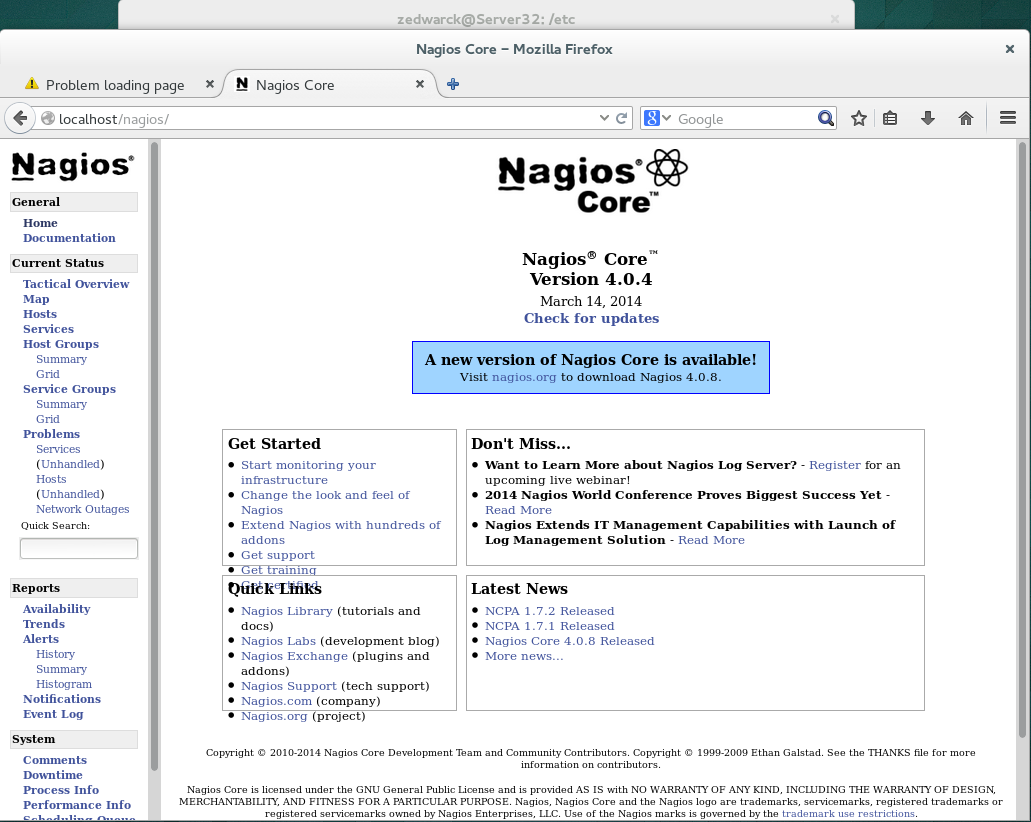
\includegraphics[width=1\textwidth]{3/nagiosrun1}
	\caption{Home Web de Nagios funcionando.}
	\label{fig:f18}
\end{figure}


%----------------------------------------------------------------------------------------
% CUESTION OPCIONAL 10
%----------------------------------------------------------------------------------------
\section{Con Ganglia haga lo mismo que con Munin.}

\begin{figure}[H]
	\centering
	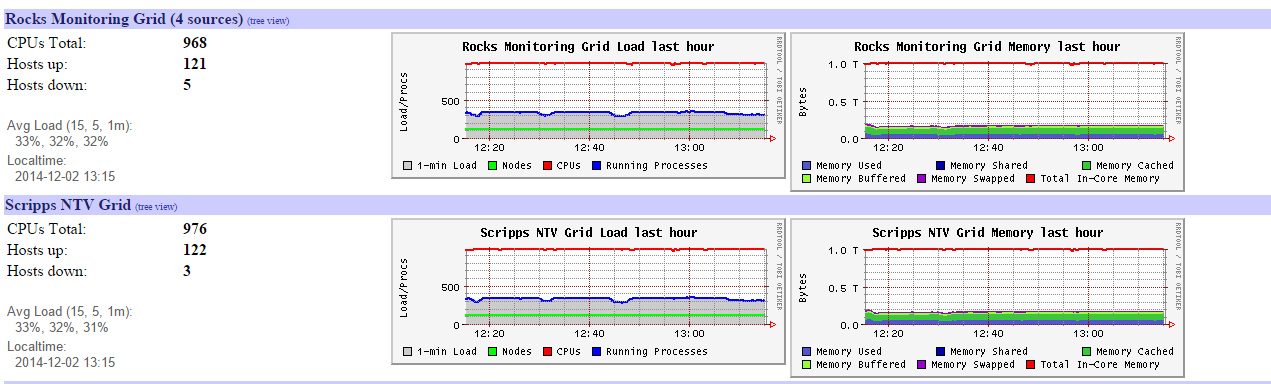
\includegraphics[width=1\textwidth]{3/co03f01}
	\caption{Monitorización de servidor de pruebas con Munin}
	\label{fig:f19}
\end{figure}



%----------------------------------------------------------------------------------------
% CUESTION OPCIONAL 11
%----------------------------------------------------------------------------------------
\section{Prueba a instalar este monitor es alguno de sus tres sistemas. Realice capturas de pantalla del proceso de instalación y comente capturas de pantalla del programa en ejecución.\cite{c09}}

Instalamos y configuramos nuestro servidor con zabbix siguiendo los pasos indicados en la cita(exceptuando el usuario de la base de datos que en nuestro caso era root).\\
Una vez instalado podemos acceder con el navegador:

\begin{figure}[H]
	\centering
	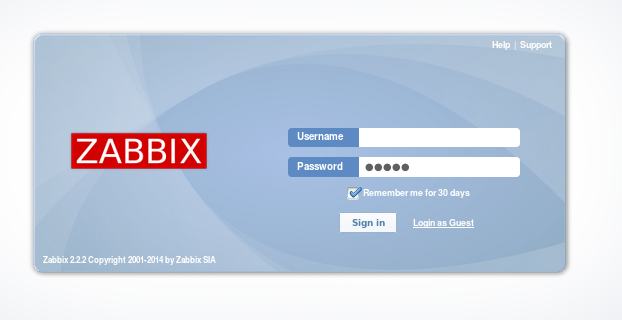
\includegraphics[width=1\textwidth]{3/co04f01}
	\caption{Pantalla de login de Zabbix.}
	\label{fig:f20}
\end{figure}

Introducimos usuario: admin y clave: zabbix, para acceder y ya tendremos la pantalla de inicio:\\
\begin{figure}[H]
	\centering
	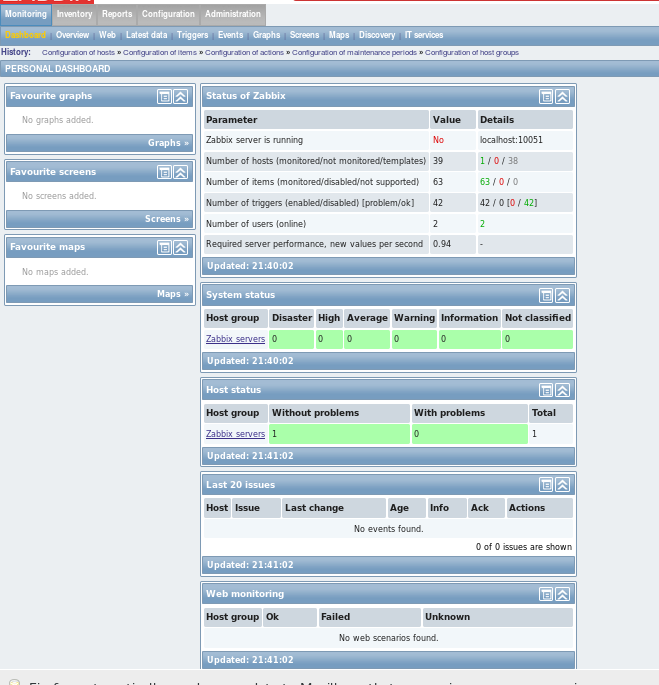
\includegraphics[width=1\textwidth]{3/co04f02}
	\caption{Pantalla Principal de Zabbix.}
	\label{fig:f21}
\end{figure}



%----------------------------------------------------------------------------------------
% CUESTION OPCIONAL 12
%----------------------------------------------------------------------------------------

\section{Pruebe a instalar este monitor en alguno de sus tres sistemas. Realice capturas de pantalla del proceso de instalación y comente las capturas de pantalla 	del programa de ejecución}

Necesitamos tener apache, php5 y mysql como prerequisito, para ello ponemos:\\

sudo apt-get install apache2 php5 mysql-server phpmyadmin\\

Una vez tengamos todo los prerequisitos, instalamos cacti:\\

sudo apt-get install cacti cacti-spine\\

Después de hacer toda la instalación ya ponemos ir a un navegador y poner como dirección: localhost/cacti

\begin{figure}[H]
	\centering
	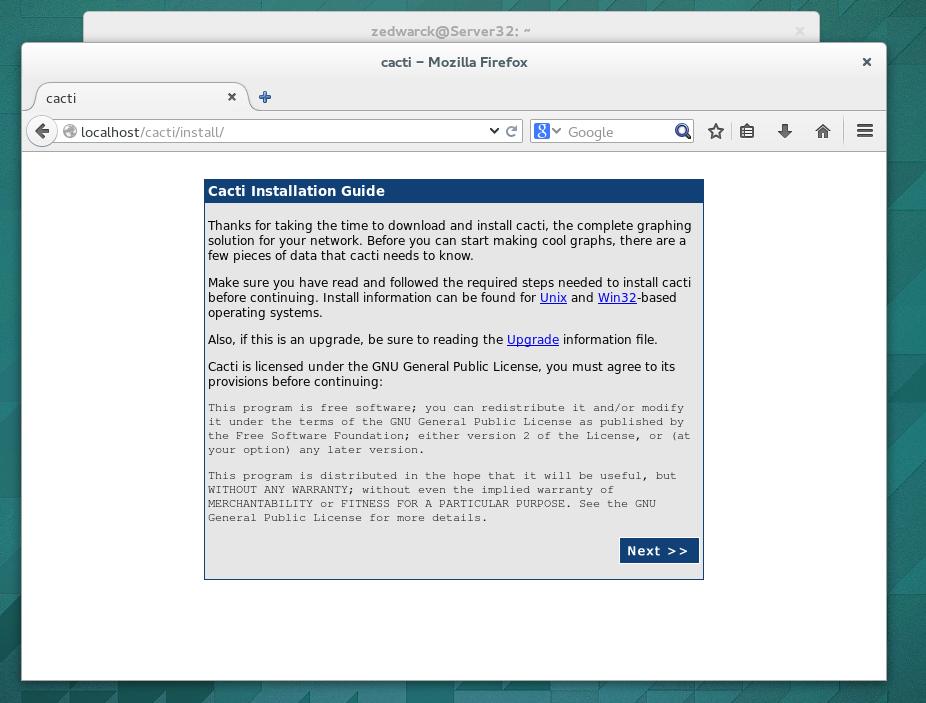
\includegraphics[width=1\textwidth]{3/co05f01}
	\caption{Pantalla inicial de preinstalación de Cacti.}
	\label{fig:f22}
\end{figure}

Pulsamos a siguiente y le decimos que queremos una nueva instalación:

\begin{figure}[H]
	\centering
	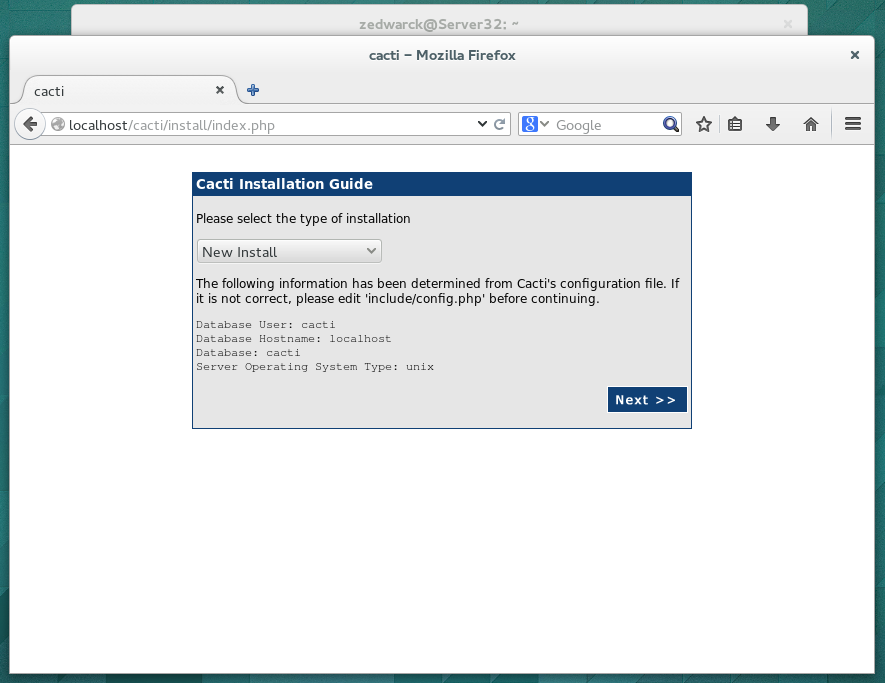
\includegraphics[width=1\textwidth]{3/co05f02}
	\caption{Opción de nueva instalación o actualización.}
	\label{fig:f23}
\end{figure}

Luego el sistema comprueba que están los archivos que necesita en sus rutas adecuadas. Pulsamos terminar para completar el proceso:

\begin{figure}[H]
	\centering
	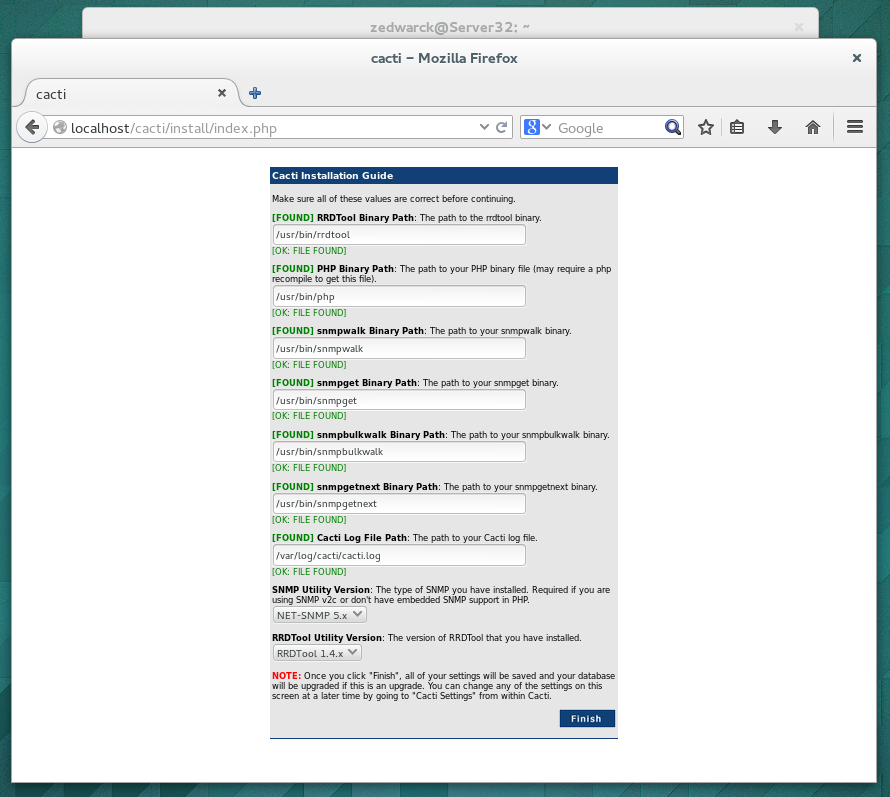
\includegraphics[width=1\textwidth]{3/co05f03}
	\caption{Comprobación de rutas en la instalación de cacti.}
	\label{fig:f24}
\end{figure}

Luego nos pide un usuario y un password que le ponemos "admin admin":

\begin{figure}[H]
	\centering
	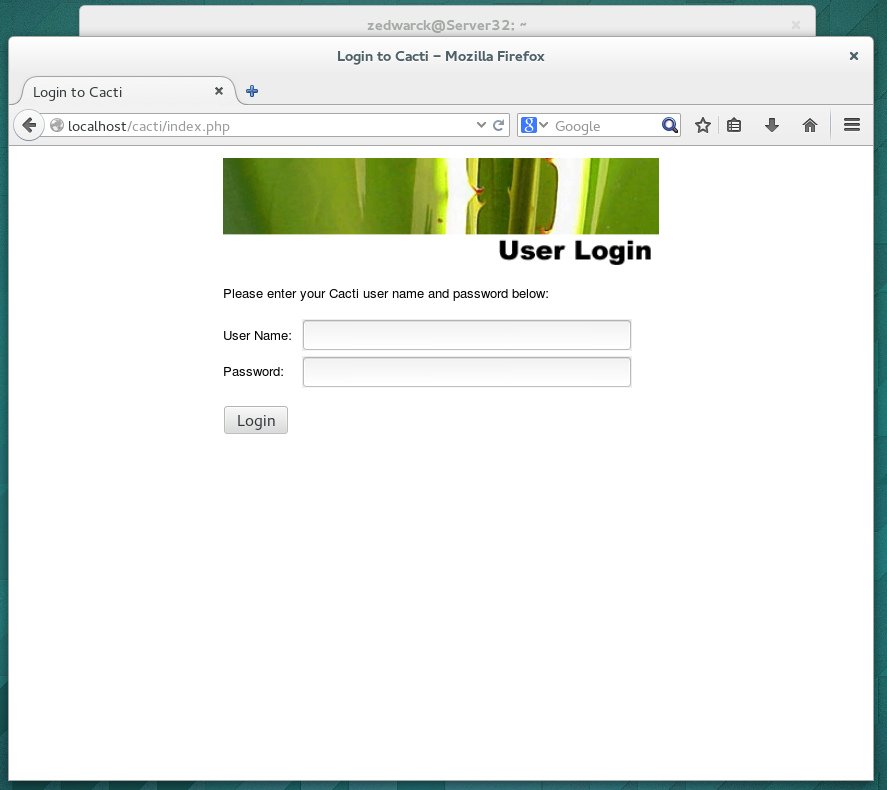
\includegraphics[width=1\textwidth]{3/co05f04}
	\caption{Login en cacti.}
	\label{fig:f25}
\end{figure}

Luego nos obliga a cambiar de password:

\begin{figure}[H]
	\centering
	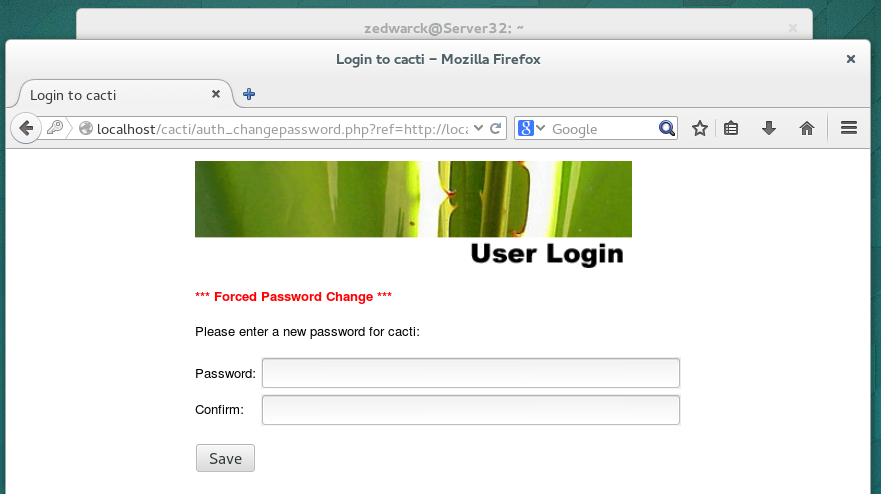
\includegraphics[width=1\textwidth]{3/co05f05}
	\caption{Cambio de password para admin en cacti.}
	\label{fig:f26}
\end{figure}

Finalmente accedemos al entorno web de cacti:
\begin{figure}[H]
	\centering
	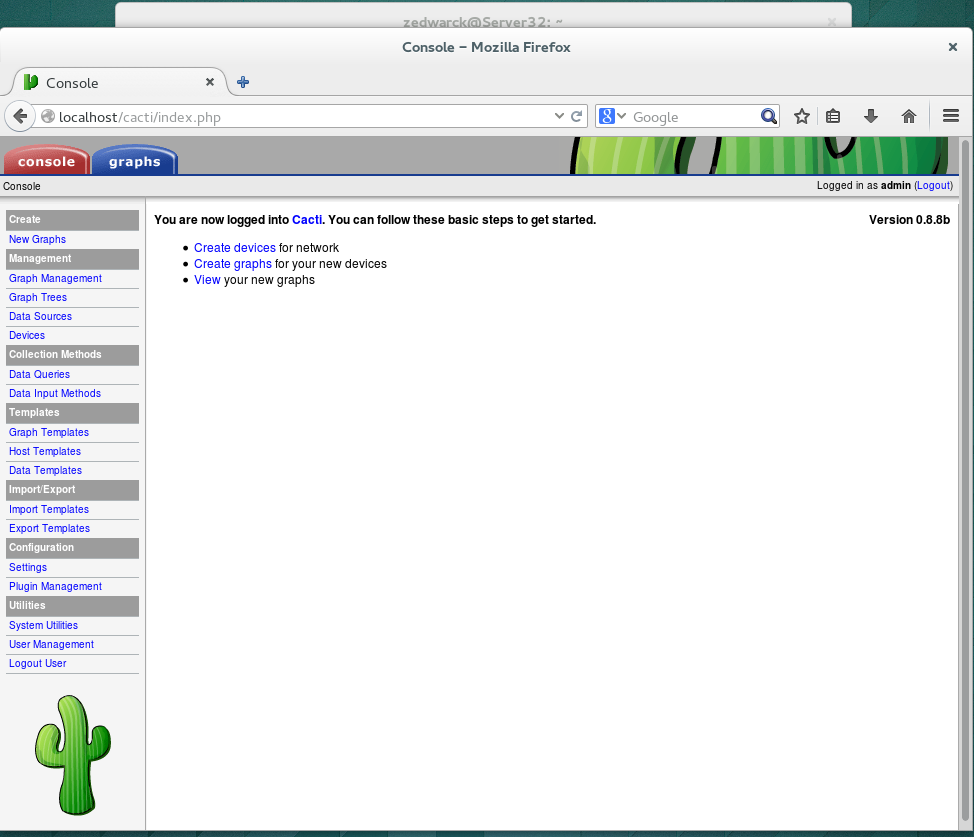
\includegraphics[width=1\textwidth]{3/co05f06}
	\caption{Home de cacti.}
	\label{fig:f27}
\end{figure}

Podemos configurar parámetros de rango de tiempo o que es lo que queremos muestrear en gráficas, en nuestro caso el uso de memoria, la carga media del servidor, usuario logueados y procesos activos:
\begin{figure}[H]
	\centering
	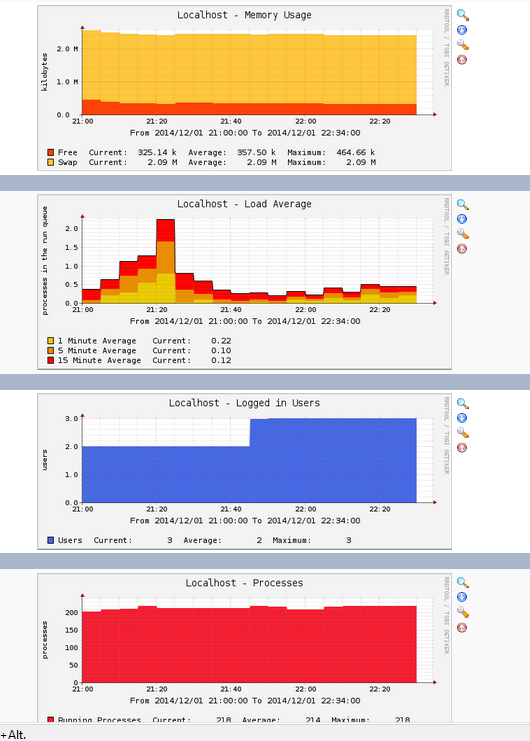
\includegraphics[width=1\textwidth]{3/co05f07}
	\caption{Gráficas de muestreo en cacti.}
	\label{fig:f28}
\end{figure}

%----------------------------------------------------------------------------------------
% CUESTION OPCIONAL 13
%----------------------------------------------------------------------------------------
\section{Desarrolle una página en C o C++ y analice su comportamiento usando valgrind.}

Mi codigo:
\begin{lstlisting}[style=C]
#include <stdio.h>
#include <stdlib.h>
#include <string.h>
#include <time.h>

int main(int argc, char **argv){

if (argc>6 || argc<5){
printf("\nERROR. Numero de parametros incorrecto. USO: %s <fila_A> <columna_A> <fila_B> <columna_B> [-v].\n", argv[0]);
exit(EXIT_FAILURE);
}

int f1 = atoi(argv[1]);
int c1 = atoi(argv[2]);
int f2 = atoi(argv[3]);
int c2 = atoi(argv[4]);

if(c1!=f2){
printf("\nERROR. Las matrices no son multiplicables. Tamano incorrecto.\n");
exit(EXIT_FAILURE);
}

int i, j, k;
int suma;
srand(time(NULL));

//Se crean las matrices y se reserva la memoria
int **A;
int **B;
int **C;

double tiempo;
struct timespec tiempoI, tiempoF;

A = (int **)malloc(f1*sizeof(int *));
for(i=0;i<f1;i++)
A[i]=(int *)malloc(c2*sizeof(int));

B = (int **)malloc(f1*sizeof(int *));
for(i=0;i<f1;i++)
B[i]=(int *)malloc(c1*sizeof(int));

C = (int **)malloc(f2*sizeof(int *));
for(i=0;i<f2;i++)
C[i]=(int *)malloc(c2*sizeof(int));


//Se rellenan con enteros aleatorios del 0 al 9
for (i=0; i<f1; i++)
for (j=0; j<c1; j++)
B[i][j] = rand()%10;

for (i=0; i<f2; i++)
for (j=0; j<c2; j++)
C[i][j] = rand()%10;


//Se multiplica
clock_gettime(CLOCK_REALTIME, &tiempoI);
for (i=0; i<f1; i++)
for (j=0; j<c2; j++){
suma = 0;
for (k=0; k<c1; k++)
suma += B[i][k] * C[k][j];
A[i][j] = suma;
}
clock_gettime(CLOCK_REALTIME, &tiempoF);
//Se muestra por pantalla la Solucion Completa
if (argc==6){
if (strcmp("-v",argv[5])==0){
for (i=0; i<f1; i++){
printf("\n");
for (j=0; j<c2; j++){
if (A[i][j]>=1000)
printf("%d",A[i][j]);
else if (A[i][j]>=100)
printf(" %d",A[i][j]);
else if (A[i][j]>=10)
printf("  %d",A[i][j]);
else
printf("   %d",A[i][j]);
}
}
printf("\n");
}
else{		
printf("Parametro opcional incorrecto.\n");
}
}
else{
tiempo = (double) (tiempoF.tv_sec - tiempoI.tv_sec) + (double) ((tiempoF.tv_nsec - tiempoI.tv_nsec) / (1.e+9));

printf("Tiempo: %8.6f\n",tiempo);
printf("Componente(0,0): %d\n",A[0][0]);
printf("Componente(N-1,N-1): %d\n",A[f1-1][c2-1]);
}

//Se libera la memoria

for(i=0;i<f1;i++)
free(A[i]);
free(A);

for(i=0;i<f1;i++)
free(B[i]);
free(B);

for(i=0;i<f2;i++)
free(C[i]);
free(C);

return(EXIT_SUCCESS);
}


\end{lstlisting}


y compilamos con:
\begin{listing}[style=consola, numbers=none]
	$ gcc -o matrices matrices.c
	\end{listing}
	
	Y finalmente ejecutamos para ver el resultado de valgrind con los parametros adecuados:
	
	\begin{figure}[H]
	\centering
	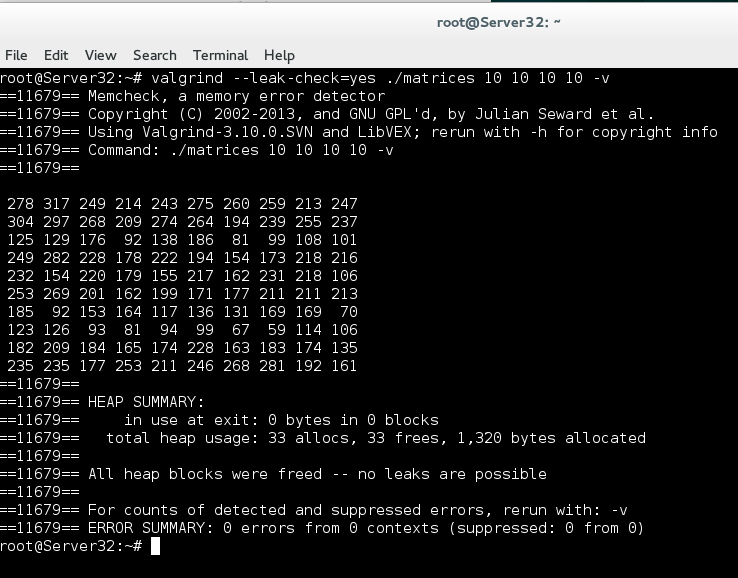
\includegraphics[width=1\textwidth]{3/co07f01}
	\caption{Resultado en consola de valgring sobre un programa de multiplicación de matrices.}
	\label{fig:f29}
	\end{figure}

\clearpage
%----------------------------------------------------------------------------------------
% CUESTION OPCIONAL 14
%----------------------------------------------------------------------------------------
\section{Seleccione, instale y ejecute uno, comente los	resultados.}

Hemos elegido un benchmark llamado "hdparm-read" que testea la velocidad de lectura de los dispositivos de almacenamiento. Incluso puede testear por dispositivos lógicos y no solo físicos.\\
Primero lo instalamos:
\begin{figure}[H]
\centering
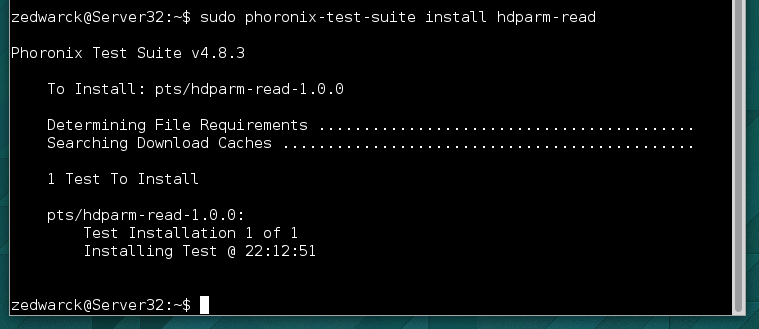
\includegraphics[width=1\textwidth]{4/po01f02}
\caption{Instalacion del benchmark hdparm-read}
\label{fig:f30}
\end{figure}


Luego lo ejecutamos:
\begin{figure}[H]
\centering
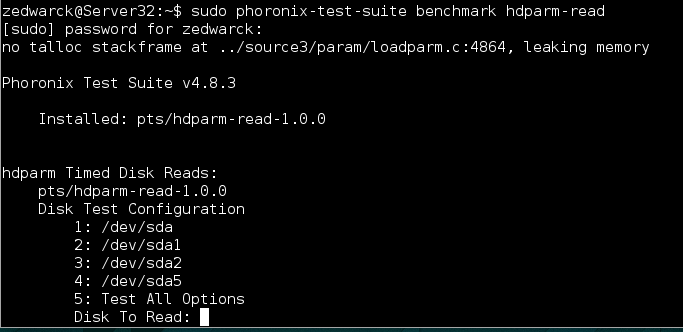
\includegraphics[width=1\textwidth]{4/po01f05}
\caption{Ejecución del benchmark hdparm-read}
\label{fig:f31}
\end{figure}

Después de elegir el sistema físico-lógico que queremos testear nos pregunta si queremos guardar los resultados del test(También nos muestra un resumen general del sistema).
\begin{figure}[H]
\centering
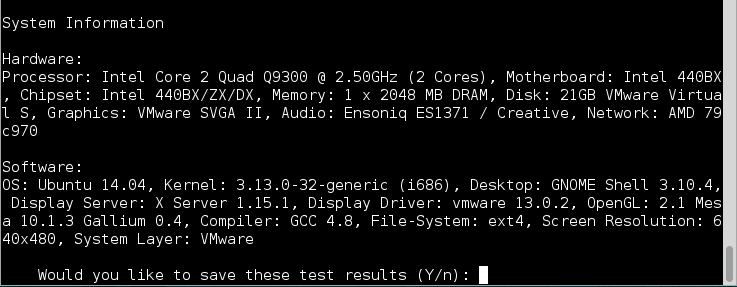
\includegraphics[width=1\textwidth]{4/po01f06}
\caption{Resumen de nuestro sistema y confirmación de guardado de datos.}
\label{fig:f32}
\end{figure}

El benchmark realiza cinco pasadas en nuestro caso:
\begin{figure}[H]
\centering
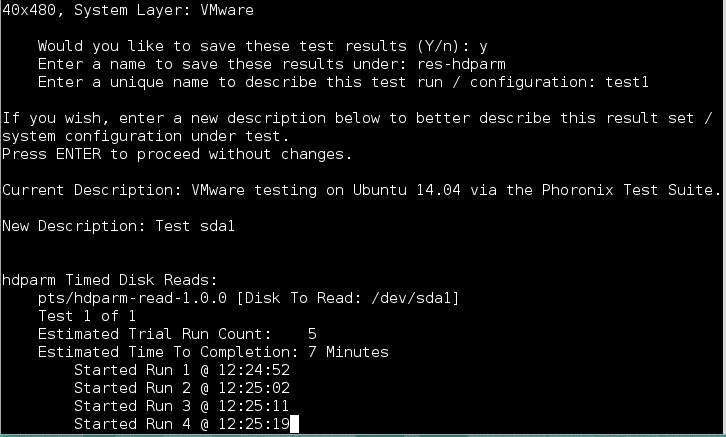
\includegraphics[width=1\textwidth]{4/po01f07}
\caption{Realización de los test de disco.}
\label{fig:f33}
\end{figure}

Finalmente nos muestra los resultados (Y nos pregunta si queremos visualizarlos en navegador.):
\begin{figure}[H]
\centering
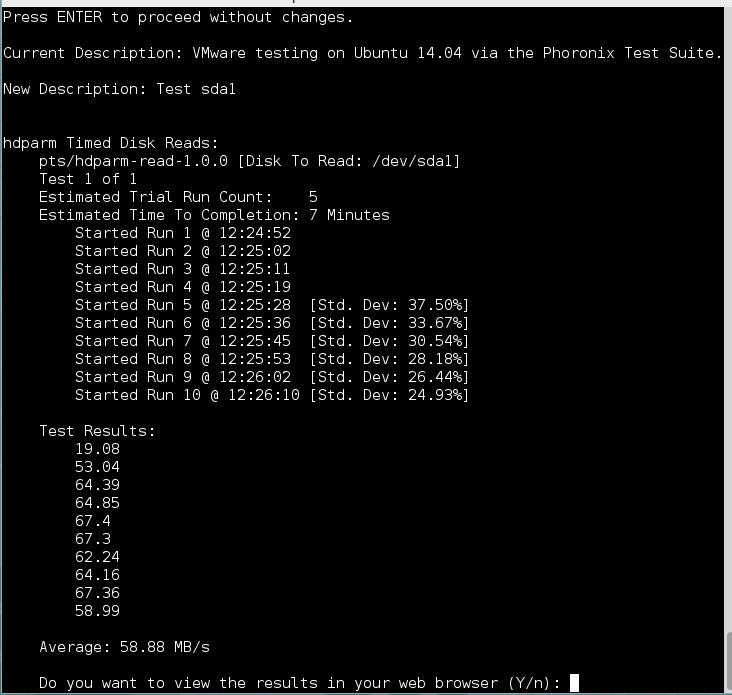
\includegraphics[width=0.65\textwidth]{4/po01f08}
\caption{Resultado del benchmark hdparm-read.}
\label{fig:f34}
\end{figure}

Resultados vistos en gráfica desde navegador.
\begin{figure}[H]
\centering
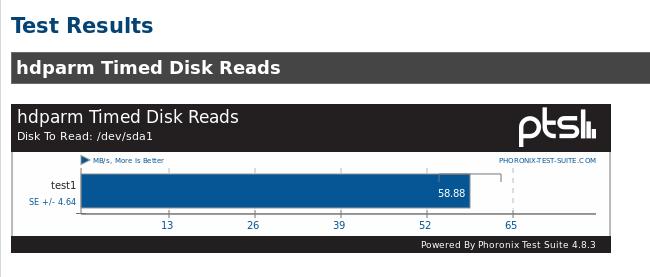
\includegraphics[width=0.6\textwidth]{4/po01f09}
\caption{Resultado del benchmark hdparm-read en gráfica.}
\label{fig:f35}
\end{figure}


%----------------------------------------------------------------------------------------
% CUESTION OPCIONAL 15
%----------------------------------------------------------------------------------------
\section{¿Qué es Scala? Instale Gatling y pruebe los escenarios por defecto. \cite{c10}}

Es un lenguaje de programación orientado a objetos. Se ejecuta en la máquina virtual de Java, por lo que puede integrarse con facilidad en los proyectos Java.\\

Para instalarlo en Ubuntu basta con: sudo apt-get install gatling\\


%----------------------------------------------------------------------------------------
% CUESTION OPCIONAL 16
%----------------------------------------------------------------------------------------
\section{Lea el artículo sobre Jmeter y elabore un breve resumen.}
El documento pretende comparar JMeter con Gatling, en la comparación tomas diversas medidas en un mismo caso simulado con 10000 usuarios y 30000 peticiones por minuto sobre un servidor web nginx.\\

Después de tomar las medidas hacen una valoración y se llega a la conclusión de que ambos son muy parecidos respecto al rendimiento. Solo destacar el nivel de procesamiento de JMeter es mayor debido a que se ejecuta sobre una maquina virtual java y eso produce un mayor volumen de procesamiento y carga de memoria RAM del servidor.

%----------------------------------------------------------------------------------------
% CUESTION OPCIONAL 17
%----------------------------------------------------------------------------------------
\section{Seleccione un benchmark entre SisoftSandra y Aida.	Ejecútelo y muestre capturas de pantalla comentando los resultados.}

Después de instalarlo lo ejecutamos y tenemos:
\begin{figure}[H]
\centering
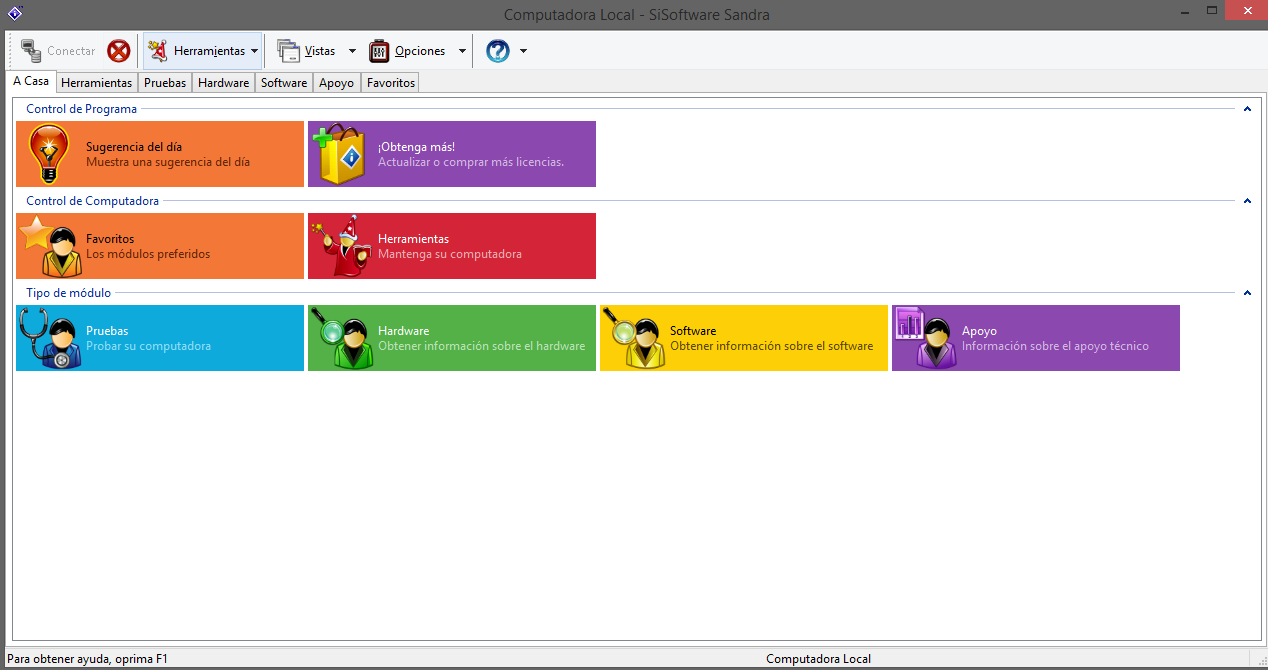
\includegraphics[width=0.8\textwidth]{4/po04f01}
\caption{Pantalla inicial de SisoftSandra.}
\label{fig:f36}
\end{figure}

Al darle a pruebas para testear nos muestra muchos tipos de tests que puede hacer a nuestra maquina. En nuestro caso elegimos que nos haga un benchmarking de la CPU y sus Gigaflops:

\begin{figure}[H]
\centering
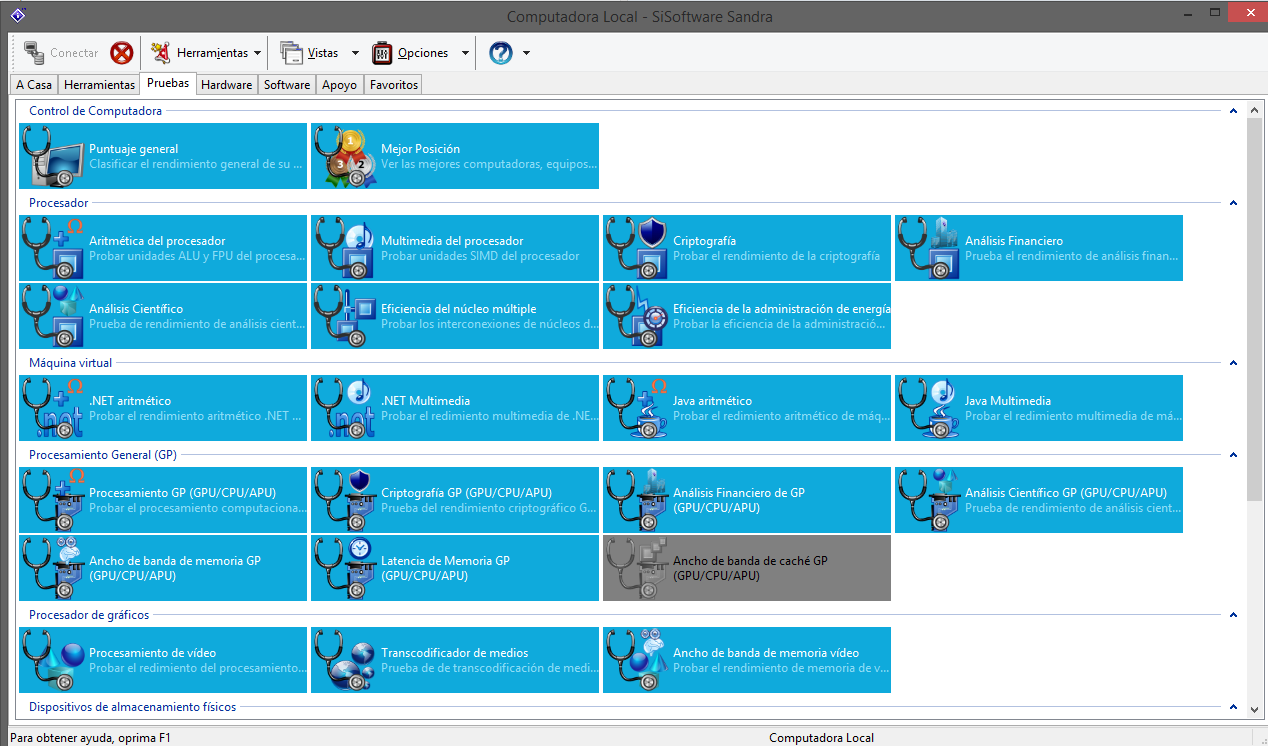
\includegraphics[width=0.7\textwidth]{4/po04f02}
\caption{Diversos test de SisoftSandra.}
\label{fig:f37}
\end{figure}


Después de un periodo de tiempo y una vez completado el test nos muestra el resumen y una grafica en la que podemos comparar con otros procesadores del mercado pudiendo elegir nosotros cuales son los procesadores de referencia:

\begin{figure}[H]
\centering
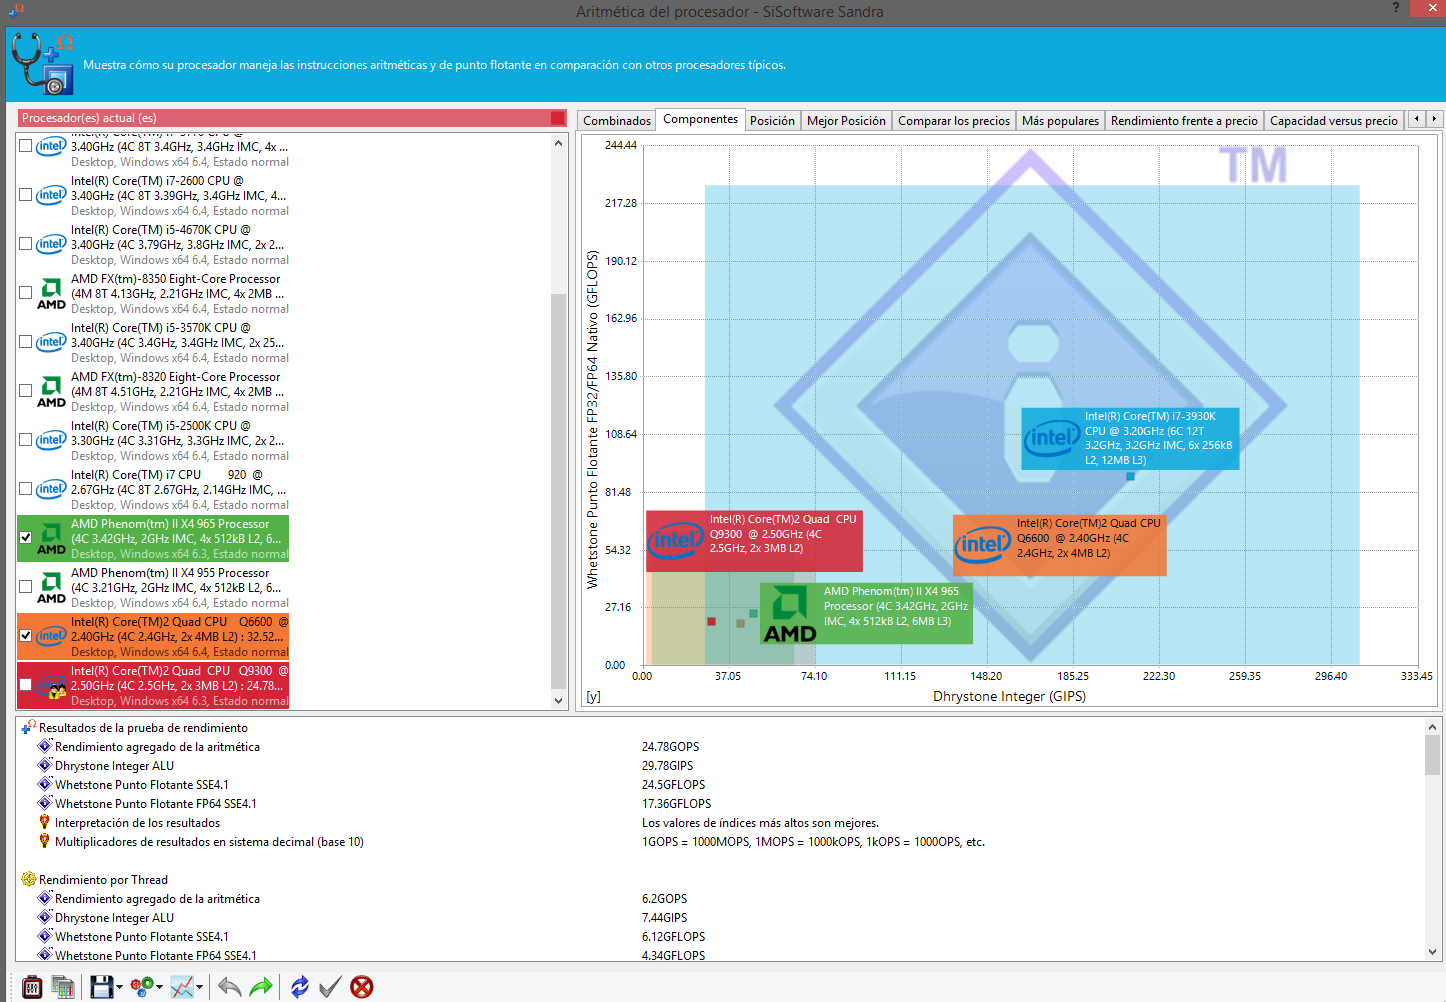
\includegraphics[width=1\textwidth]{4/po04f03}
\caption{Resultado de testear la CPU con SiSoftSandra.}
\label{fig:f38}
\end{figure}





\clearpage
\bibliography{citas} %archivo citas.bib que contiene las entradas 
\bibliographystyle{plain} % hay varias formas de citar


\end{document}